% !TEX root = meca1321-synthesis.tex

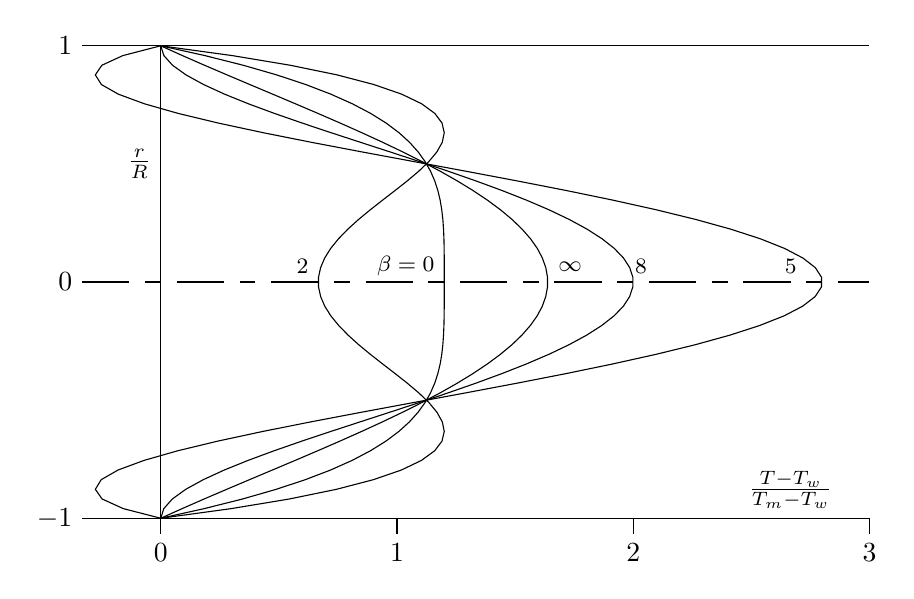
\begin{tikzpicture}
  \draw (0,-3) -- ++(0,6);
  \draw (-1, -3) node [left] {$-1$}-- ++(10,0);
  \draw (-1, 3) node [left] {$1$}-- ++(10,0);
  \draw [dash pattern= on 0.6cm off 0.2cm on 0.2cm off 0.2cm] (-1,0) node [left] {$0$} -- ++(10,0);
  \foreach \i in {0,...,3}
  {
    \draw (\i*3, -3) -- ++(0, -0.2) node [below] {$\i$};
  }
  \foreach \i in {0, 2, 5, 8, 1000}
  {
    \draw [domain=-1:1, samples=50] plot ({3*((1-(\x)^(4)) - 0.125*\i*(3-4*(\x)^(2) + (\x)^(4)))/((5/6)-(11/48)*\i)},{3*\x});
  }
  \draw (3.6,0.2) node [left] {\footnotesize$\beta=0$};
  \draw (2,0.2) [left] node {\footnotesize$2$};
  \draw (5.2,0.2) node {\footnotesize$\infty$};
  \draw (6.1,0.2) node {\footnotesize$8$};
  \draw (8,0.2) node {\footnotesize$5$};
  \draw (0, 1.5) node [left] {$\frac{r}{R}$};
  \draw (8, -3) node [above] {$\frac{T - T_w}{T_m - T_w}$};
\end{tikzpicture}
